\chapter{Conclusion}
\label{chapter:conclusion}

This work showed how PCG is important in game design and how the price of game development has been increasing throughout the years. To aid in that matter, it proposed the development of a PCG system to generate random cave-like maps that are similar to real-world caves. Finally it evaluated this system through a survey.

One of the biggest challenges faced was the research for criteria on what makes a good map, that can be seen on Section \ref{sec:goodmap}. Most of the related work we found focused on video-game \emph{levels}, which also contain additional elements like enemies and treasures. Due to this difficulty we decided to also adopt the metrics found in \textcite{carvalho:2016} to evaluate players' motivation to explore game levels in educational games, which, in turn, is an adaptation of the ARCS model measurement tool found in \textcite{keller:1987}. To meet our ends, the tool from \textcite{carvalho:2016} was adapted to verify players' perception on our auto-generated caves, which demanded a pre-test of the questionnaire to verify if it indeed attended our needs. In this sense, the evaluation method for generated maps proposed on this work can be further reused by others with little to no adaptation.

The creation of the system required knowledge from different areas and the use and adaptation of many algorithms. Our system has many user-defined parameters, which is a positive trait for map generation, since it allows for a larger variety of maps to be created. Even though the work focused on cave-like maps, by changing the used tiles the system can generate maps like forests, open fields, rivers, etc. Figure \ref{fig:river} shows a procedurally generated river, also created with the use of the system.

\begin{figure}[h]
    \caption{River generated by the system.}
    \centerline{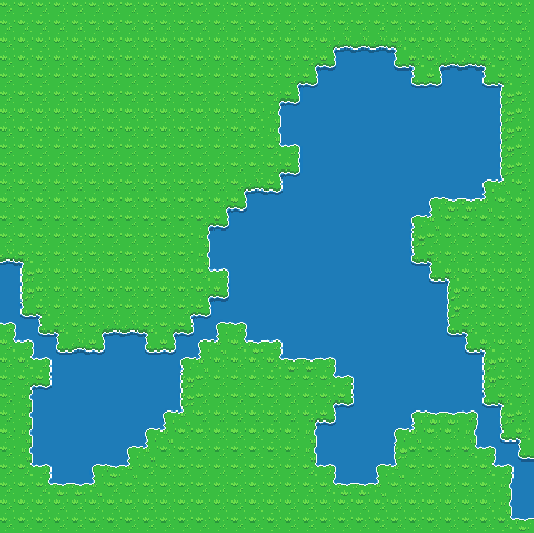
\includegraphics[width=6cm]{images/river.png}}
    \legend{Source: Image provided by author}
    \label{fig:river}
\end{figure}

The survey was answered by 163 participants, most of them from the age group that composes the average gamer and familiar to 2D top-down games. From the 12 questions, 9 achieved satisfactory results while 3 did not. Out of these results we found that, even though the structure of the maps resembles natural caves, the maps were not found to be much similar to 2D representations of real caves.

Finally, as a future works, the system could be turned into an Unity tool, that can then be used to create full games. The generation of rivers can be expanded on, by comparing them to real-life rivers and evaluating with a similar survey. The generation of maps can be changed to a level-generator, where the system wouldn't only generate the map but also place enemies, treasures, hidden passages etc. A deeper analysis of the questions regarding the ARCS model can be done to better evaluate the motivation to explore given to players by our maps.